% The cliff callback + the conflation fix (dynamics error vs value extrapolation).
% Reuses the same cliff image as the model-based failure section.

\begin{frame}{The Cliff, One Last Time}
\centering
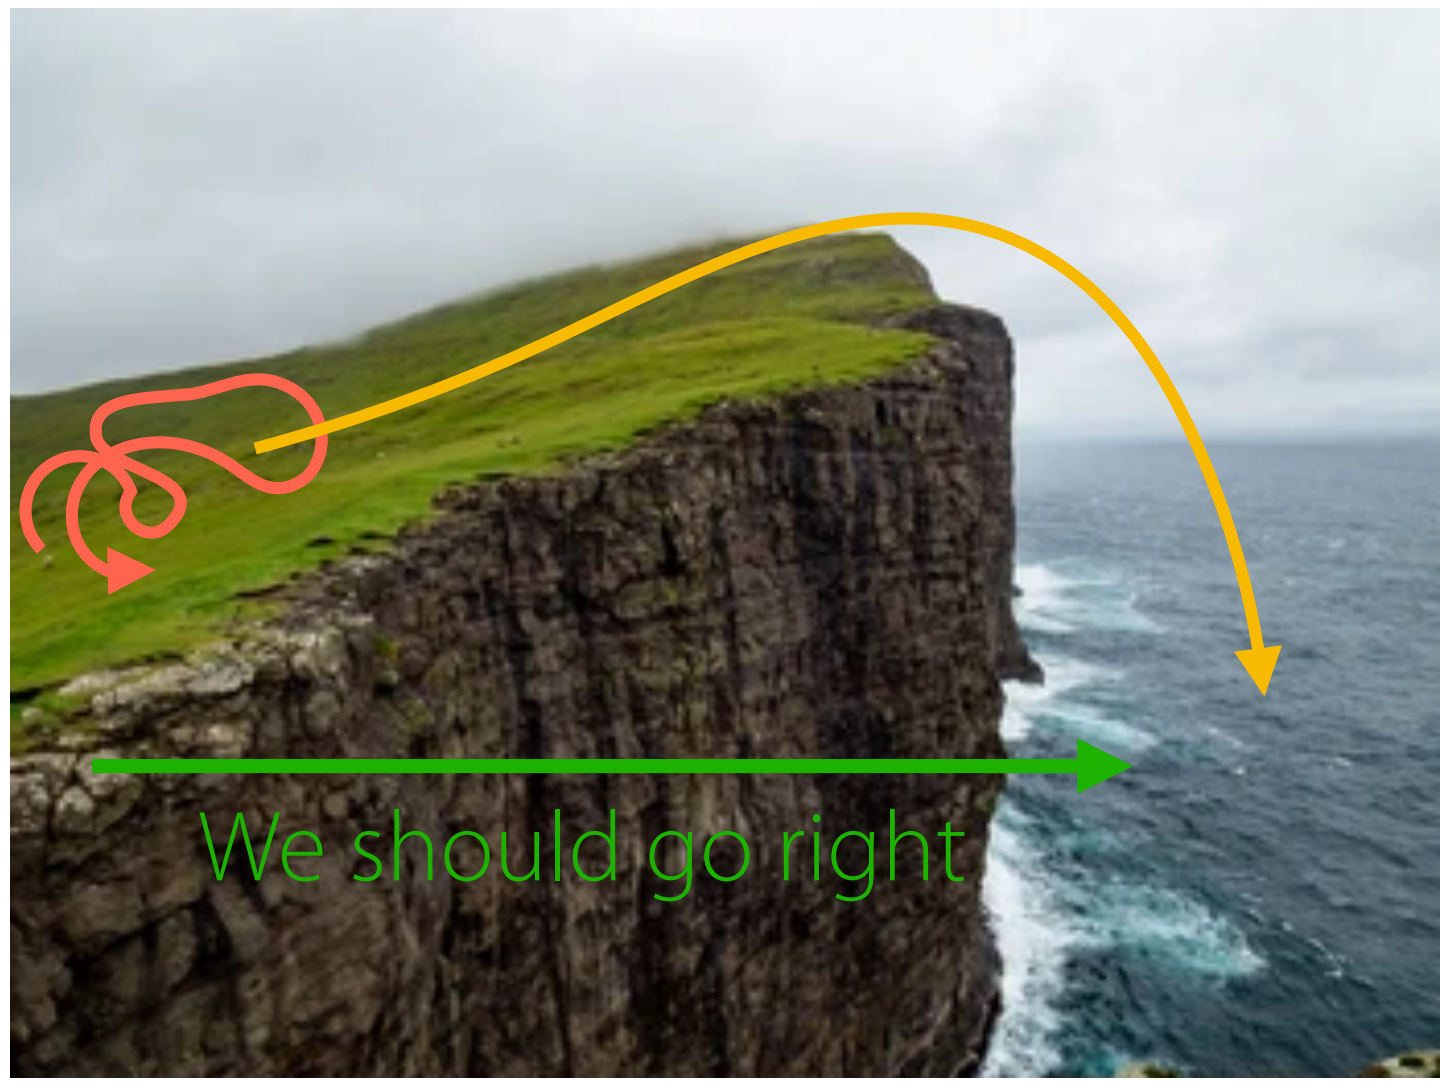
\includegraphics[width=0.36\textwidth]{images/model-based-rl/figures/cliff-fail.jpg}
\begin{itemize}
    \item Part 1's fix for distribution mismatch was to \emph{execute, observe,
          re-train}: go collect data where the model was wrong
\end{itemize}
\end{frame}

\begin{frame}{The Cliff, One Last Time}
\centering
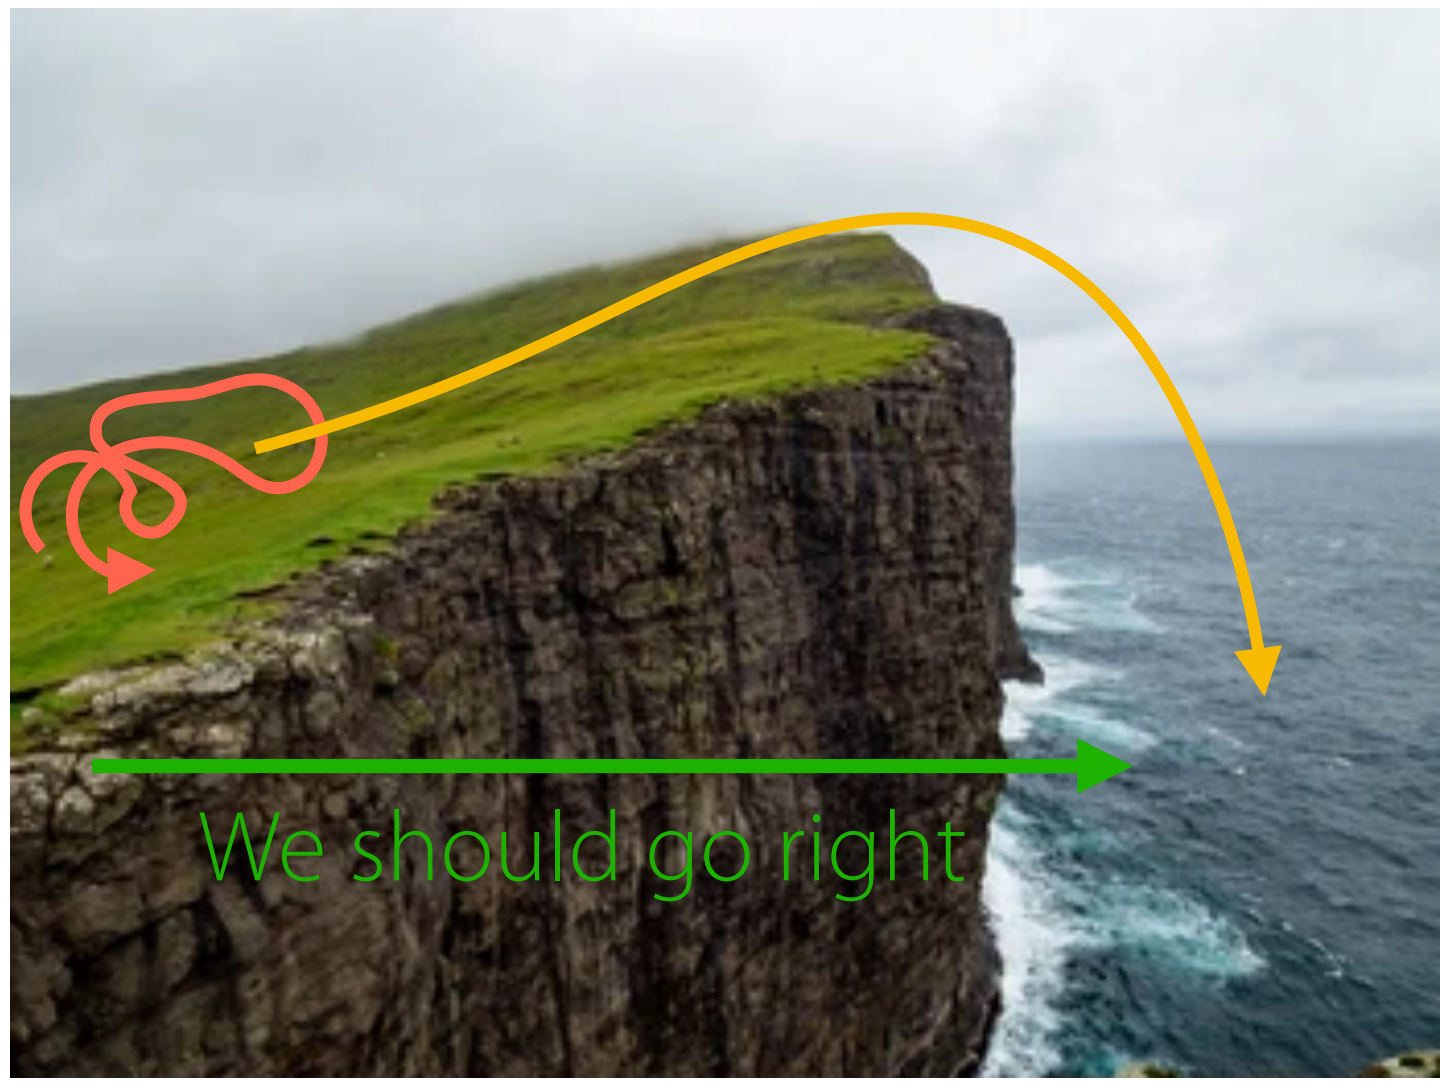
\includegraphics[width=0.36\textwidth]{images/model-based-rl/figures/cliff-fail.jpg}
\begin{itemize}
    \item Part 1's fix for distribution mismatch was to \emph{execute, observe,
          re-train}: go collect data where the model was wrong
    \item Offline RL is \textbf{exactly this problem, with the fix forbidden}
\end{itemize}
\end{frame}

% === Same disease, different organ (the conflation fix) =================
\begin{frame}{Same Disease, Different Organ}
\definecolor{oblue}{RGB}{16,53,103}
\definecolor{ogreen}{RGB}{106,168,79}
\definecolor{ored}{RGB}{158,28,38}
\centering
\begin{tikzpicture}[font=\scriptsize, >={Stealth[length=2.4mm]},
    obox/.style={rounded corners, align=center, thick, inner sep=4pt}]
    % model-based pipeline
    \node[obox, draw=oblue, fill=oblue!12]                     (m1) {model wrong\\off-distribution};
    \node[obox, draw=ogreen, fill=ogreen!12, right=0.7cm of m1] (m2) {collect data there,\\re-train};
    \draw[->, thick] (m1) -- (m2);
    \draw[->, thick, ogreen!70!black] (m2.north) to[bend right=45] (m1.north);
    \node[oblue, font=\scriptsize\bfseries]
      at ($(m1.north)!0.5!(m2.north)+(0,0.95)$) {Model-based (part 1)};
    % offline pipeline
    \node[obox, draw=oblue, fill=oblue!12, right=1.7cm of m2]  (o1) {$Q$ wrong\\off-distribution};
    \node[obox, draw=ored,  fill=ored!12,  right=0.7cm of o1]  (o2) {collect\\more data};
    \draw[->, thick] (o1) -- (o2);
    \draw[ored, very thick] (o2.south west) -- (o2.north east);
    \node[oblue, font=\scriptsize\bfseries]
      at ($(o1.north)!0.5!(o2.north)+(0,0.95)$) {Offline (part 2)};
\end{tikzpicture}
\begin{itemize}
    \item Careful, the failure \emph{mechanisms} differ:
    \item The cliff was a \textbf{dynamics-model} error: $f_\phi$ predicted the
          wrong next state
    \item Offline RL's core failure is \textbf{value extrapolation}: $Q$ invents
          values for actions the data never contains; it bites \emph{even
          with perfect dynamics}
    \item Same disease (distribution shift), different organ (the model vs.\ the
          value function)
\end{itemize}
\end{frame}
